\documentclass{article}

\usepackage{graphicx}
\usepackage{amssymb}
\usepackage{amsmath}
\usepackage{amsfonts}
\usepackage{verbatim}
\usepackage{indentfirst}
\usepackage{amsthm}
\usepackage{framed}
\usepackage{enumitem}

\usepackage{titling}

%%%%%
% Setup
%%%%%
\newcommand{\p}{\mathbb{P}}
\newcommand{\e}{\mathbb{E}}

% Margins
\setlength{\textwidth}{6.5in}
\setlength{\oddsidemargin}{0in}
\setlength{\evensidemargin}{0in}

%\setlength{\droptitle}{-0.5in}

\def\squarebox#1{\hbox to #1{\hfill\vbox to #1{\vfill}}}
\newcommand{\qedbox}
{\vbox{\hrule\hbox{\vrule\squarebox{.667em}\vrule}\hrule}}
%\newcommand{\qed}               {\nopagebreak\mbox{}\hfill\qedbox\smallskip}

\title{MapReduce System (MRS)\\
{\large 6.945 Final Project - Spring 2014}}
\author{Lars Johnson (larsj@mit.edu) \\ Gurtej Kanwar (gurtej@mit.edu)}
\date{May 12, 2014}

%%%%%
% Document
%%%%%
\begin{document}
\pagestyle{myheadings}
\maketitle

\markright{MapReduce System - 6.945 Final Project - Lars Johnson}

\section{Overview}

We looked into the problem of building a system to work with data sets
as a fundamental type. This problem was inspired by the Map Reduce algorithm:
a system which performs a distributed map operation on a data set, followed
by a reduce. We took this problem and generalized to stateful multi-maps on data
sets. The ultimate goal was to build a system which allowed the user to
use MIT Scheme to assemble a network of data-set operations, feed data set
inputs at various points in the network, and extract processed output from
the network. We successfully built a system which provided user-facing functions
to build the graph and set inputs and outputs. The user can do this both interactively
through a custom REPL environment and by defining a thunk to perform construction
and input which is executed in the default REPL by our run-computation function.

\subsection{Basic Example}

See Figure 1 for a basic example of using our system to perform the
map-reduce operation of determining word frequencies over a set of documents.
\begin{figure}[h!]
  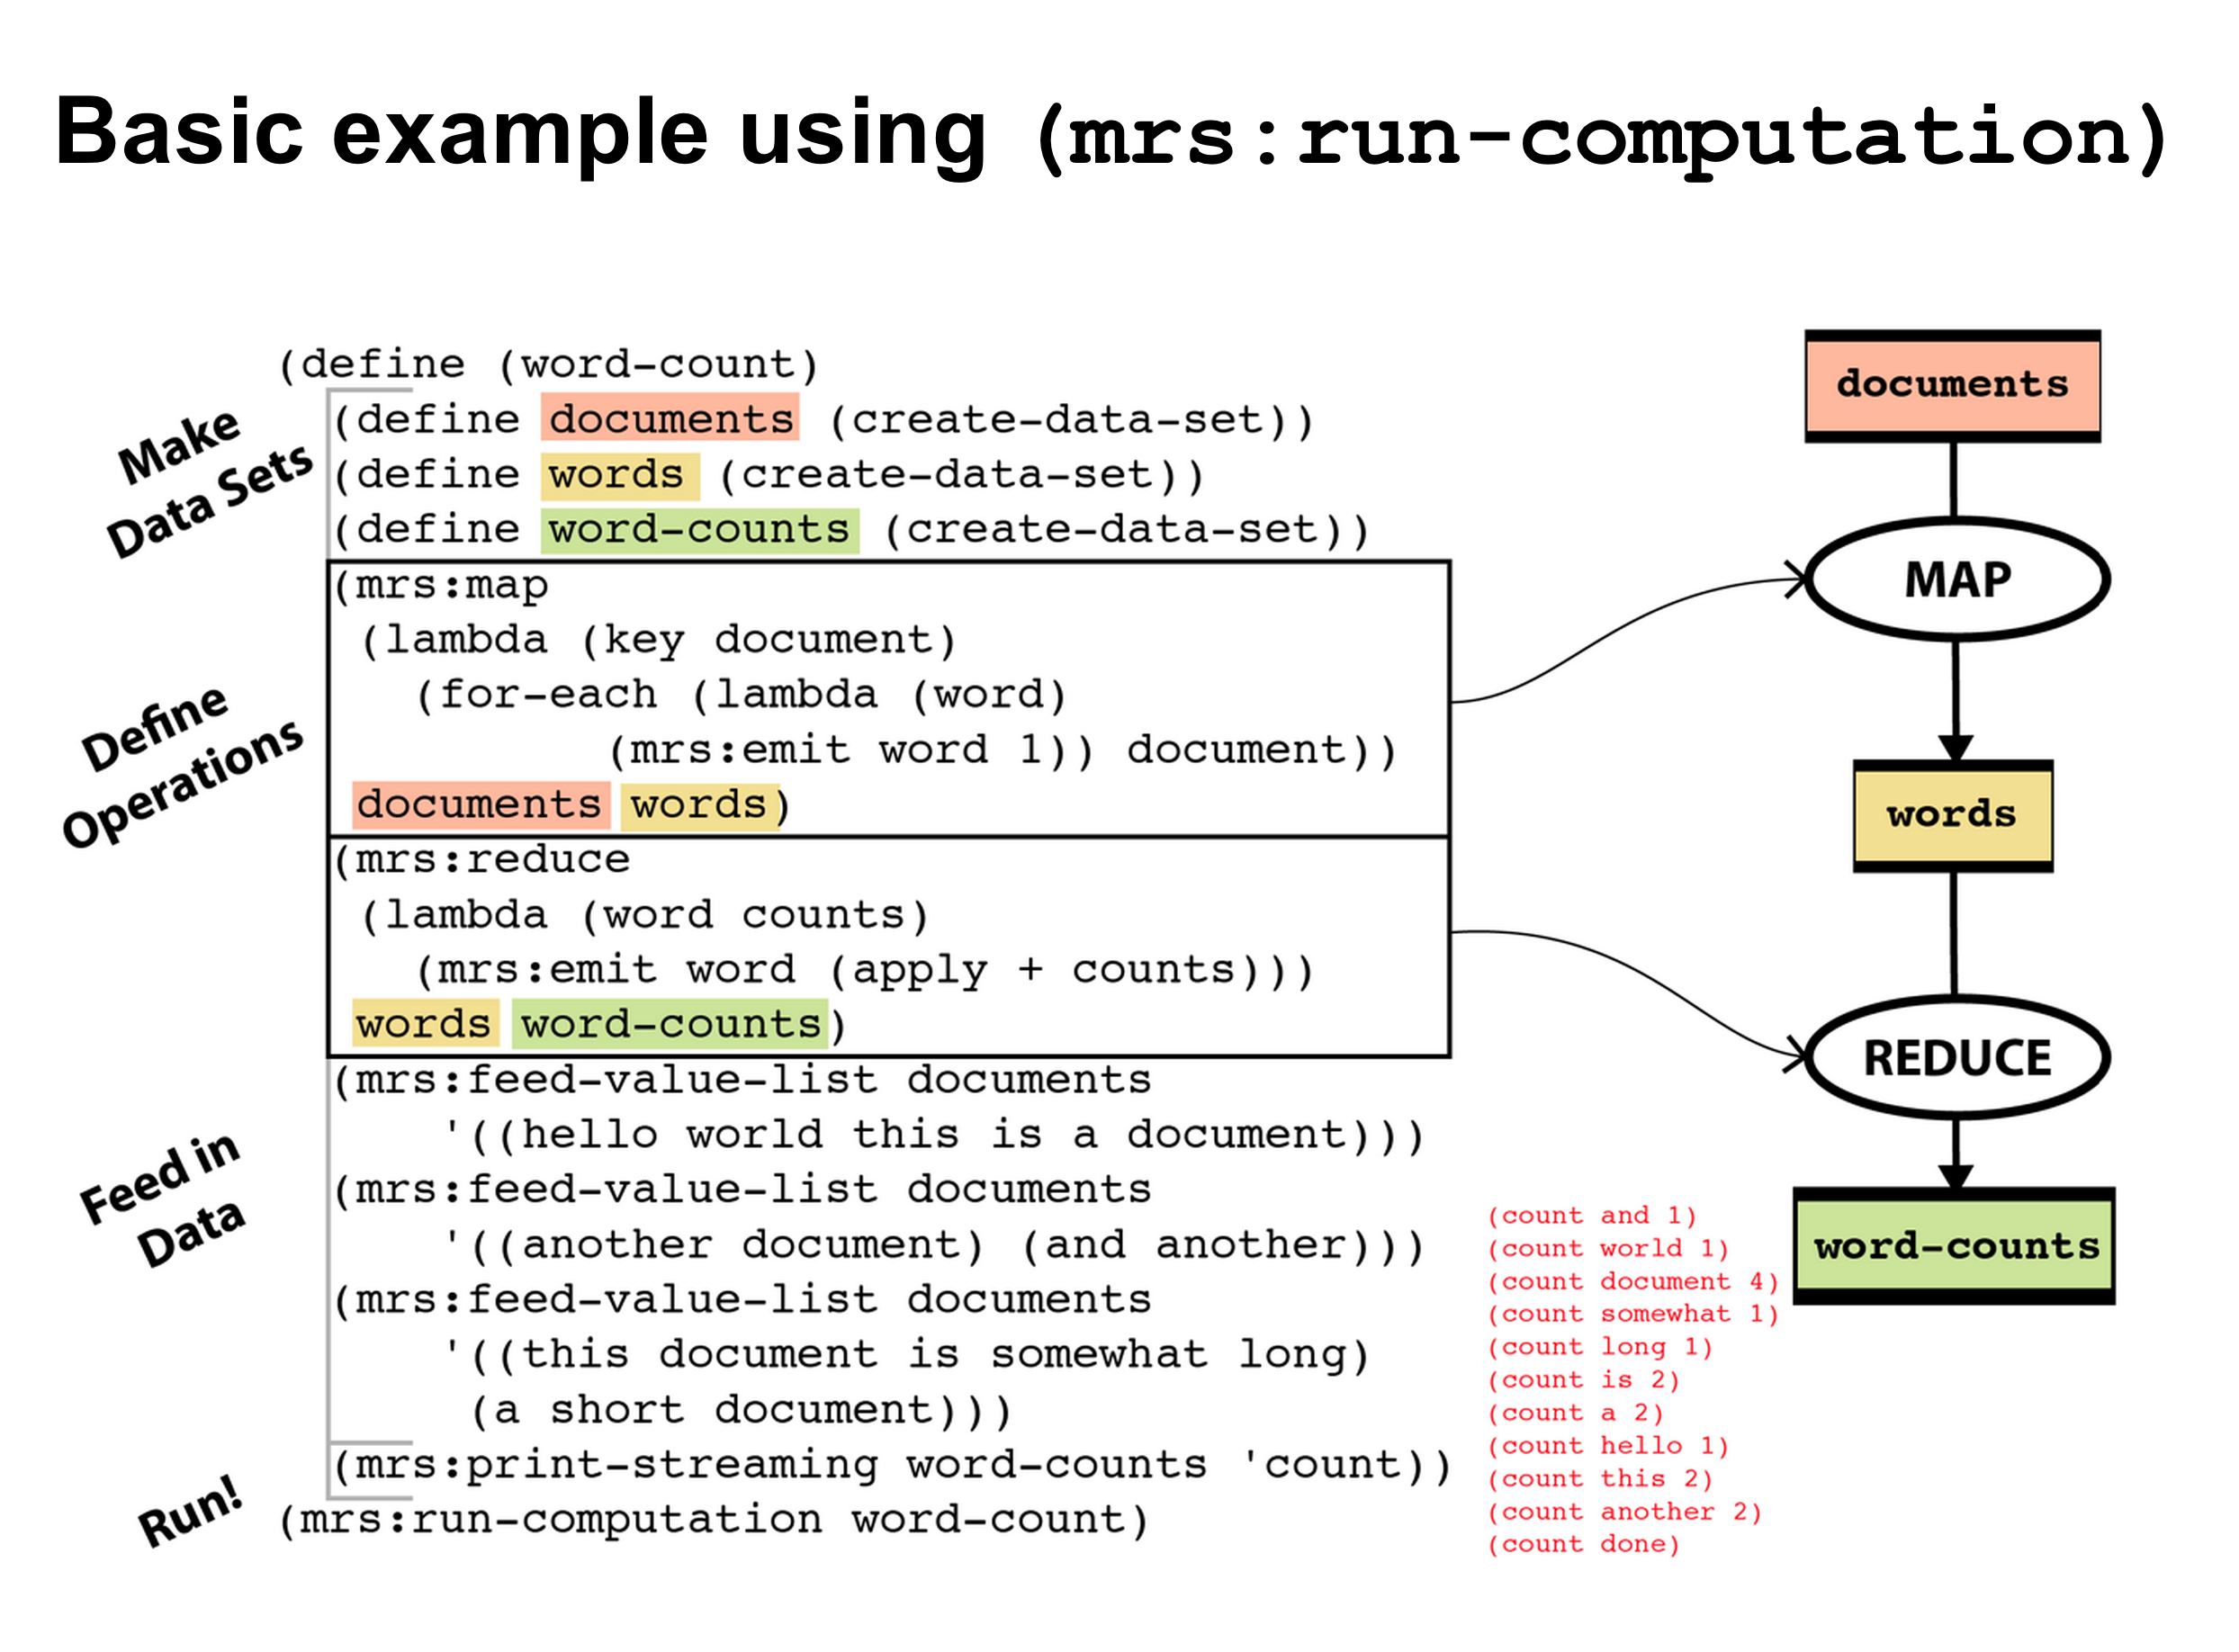
\includegraphics[width=\textwidth]{basic-example.png}
  \caption{\emph{\small A basic example of using our system to
      performe the map-reduce operation of counting the number of
      words present in a set of documents}}
\end{figure}

\section{Context}

\subsection{Definitions}

\textbf{Data set:} A multi-set of (key,value) pairs. Because this is a multi-set, multiple
copies of the same key can exist.

\textbf{Multi-map operation:} A function from a single (key,value) pair to zero or more
(newkey, newvalue) pairs. As an example, both the map and filter operations are subsets
of this abstraction.

\textbf{Stateful multi-map operation:} A function from a single (key,value) pair and previous
state to zero or more (newkey, newvalue) pairs and new state. This is a slightly broader
abstraction than multi-map, which allowed us to cover all operations which we were interested
in implementing.


\subsection{MapReduce Background}

The inspiration for this project came from the MapReduce algorithm developed by
Jeffrey Dean and Sanjay Ghemawat at Google in 2004. The algorithm operates on a
single input data set, by first performing a distributed \textbf{map} over all of
the input (key,value) pairs, then aggregating values by keys and performing a
distributed \textbf{reduce} over each
of the lists of aggregated values.

A canonical example of a MapReduce operation is
word counts from a list of documents. To construct this MapReduce we define the
map to act on (id, document) pairs and output (word, count) pairs, and we define
the reduce to receive the aggregated word count pairs (word, [count1, count2, ...])
and output a single (word, count) pair. The implementation of map in this example
iterates over the words of the document and emits a (word, 1) pair for each word
it sees. After aggregation, the reduce operation simple has to iterate through the
given counts and sum them to output the final counts.

The advantage of framing a computation on a data set as a MapReduce operation
is that the definitions of map and reduce can completely ignore the massively
distributed nature of the actual computation and focus on the actual operations
being applied to the data. As demonstrated by Google, this has been quite
successful for performing large-scale calculations that are farmed out to thousands
of machines.


\subsection{Extending MapReduce}

While MapReduce was an interesting problem, it is a very specific method of
operating on data sets. Our goal from this project was to extend this paradigm
to a more general system of computation on data sets as fundamental units of
data. We looked at the MapReduce problem and came up with a generalization
of the operations involved to \emph{stateful multi-map} operations.

Both map and reduce are actually non-stateful multi-map functions: map accepts a (key,value) pair
and emits zero or more (newkey, newvalue) pairs in a (potentially) different
domain; reduce accepts a (key,valuelist) pair and generally emits exactly
one (newkey,newvalue) pair as output. The hidden third operation, the aggregation
step, is trickier to generalize. The aggregation step requires information
from all of its inputs at once to generate an output. This does not fit the 
mould of a simple multi-map function, since each (key,value) pair by itself
does not provide enough information to aggregate. We thus decided to broaden our
generalization to stateful multi-map operations. By allowing state, map, reduce
and aggregation could all be thought of as specific types of stateful multi-map
functions. There are several other common data-set operations that fall into this category
as well: filter a data set or combining two data sets, for example.


\section{Our System}

This section describes some high-level aspects of our system. See the attached code and comments for more specifics about our system implementation.

\subsection{Key Ideas}

Our system is built on four key ideas:

\begin{itemize}

\item Enable users to build a graph of data sets connected by operations

\item Allow them to feed data into data sets and it will be processed in a distributed manner across a worker pool

\item Create an abstraction system to allow for streaming implementations

\item Provide programmers with a combinator-like family of reusable parts

\end{itemize}

\subsection{System Architecture}

\begin{figure}[h!]
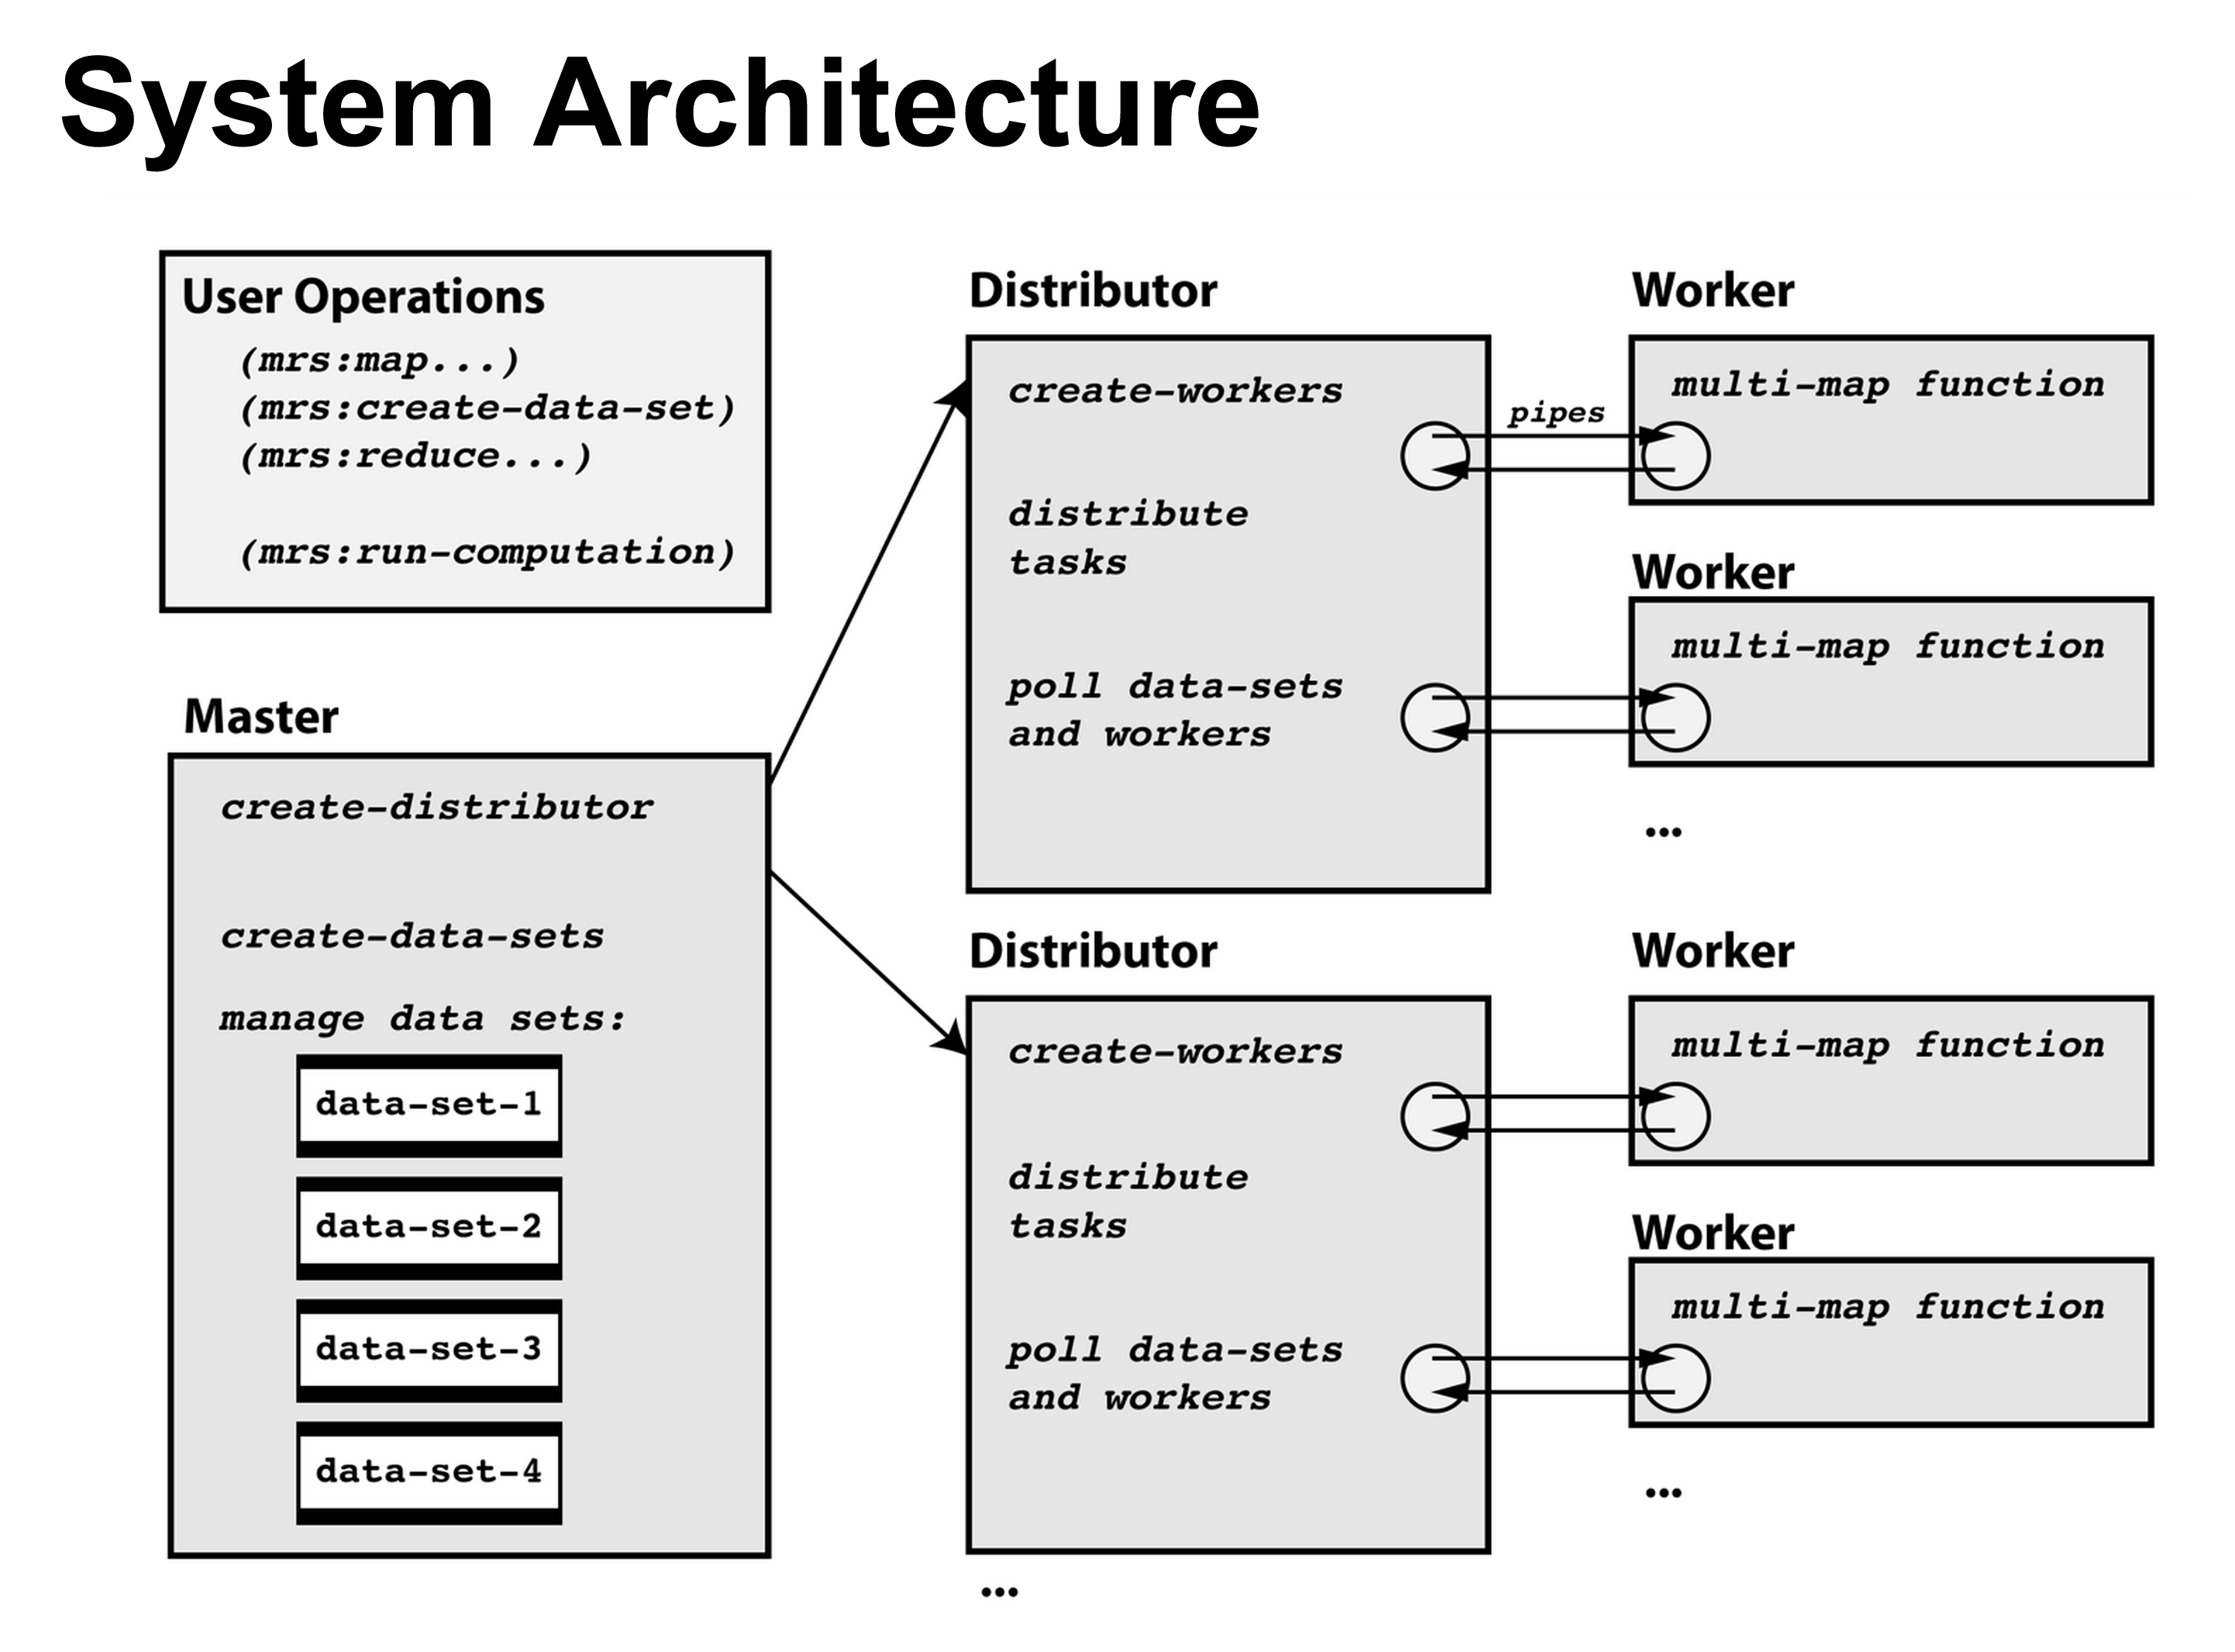
\includegraphics[width=\textwidth]{system-arch.png}
  \caption{\emph{\small The high-level architecture of our four main
      components (User Operations, Masters, Distributors, Workers).}}
\label{piefig}
\end{figure}

Our MapReduce System is comprised of four main components (See diagram
2). On the top level, a set of user operations such as (mrs:create-data-set)
(mrs:map), (mrs:reduce), and (mrs:feed-data) enable a user
of the system to specify a dataflow network and feed data into
it. Executing such specifications from within a
(mrs:run-computation) call directs a master process to allocate the
threads and spawn a distriobutor task for each requested
computation. These distributors coordinate execution of the function
and will spawn a number of worker threads to perform the exeuction.

\subsection{Communication Details}

A key component of developing such a system is managing communications
betweent various tasks. We used conspire:threads to provide
multi-tasking behavior for the tasks and used both non-blocking pipes
and data-sets to coordinate between systems. 

The non-blocking pipes mirror the standard pipes used conspire:threads
and consist of alocked queue. They are used as our demo means
for communiczating between small groups over long ranges.

Our main ``Data Set'' objects were implemented as multi-reader
multi-writer queues of elements. These data sets were abstracted
behind a generic get-reader / get-writer which allowed us to quickly
explore a variety of useful implementations (see below).

\subsection{Flexible Implementations}

Many of these components were designed with a focus on flexibility to
admit several possible different implementations.

\subsubsection{Pipes} 

For the inter-process communication, we pass data between our
distributors and workers via simple queued pipes. However, our data
abstraction of ``send message to worker'' and ``Get message from
worker'' could easily be reimplemented to use network / TCP
communications to communicate with an actual distributed system of computers.

\subsubsection{Data Sets}

For the communication between operators, we developed a handful of
different data-sets that could be used for passing information from
one operation to another. Our data sets primarily consisted of
limited-sized queues that transferred partially-processed data from
to-computation. We provided three types of data-sets that users can
construct to perform diferent purposes. All three of these are
accessed via a friendly officer presence:

\begin{description}

\item[Multi-Reader-Queue Data Set] \hfill \\
The main class of Data Set used in the system is based on a
multi-reader queue we built. This queue is aware of how many readers
it has and manages pointers representing each reader's location. Data
set elements remain in the queue until all readers have read the
element. 

\item[Output Data Set] \hfill \\
The user can specify a (single) output data set in the computation
network. This data set is special in that it passes the data it
receies back to the original caller of (mrs:run-computation...). If
the user specifies a callback function to run-computation, data set
results will be passed as (k v) arguments to the callback. Otherwise,
the output data set will enable (mrs:run-computation...) to block on
the computation until the data set is complete and is returned to the user.

\item[File Writer Data Set] \hfill \\
The file-writer data set mirrors that of the output data set in that
it provides a means of returning data set results to the user. Upon
creation, users specify a filepath and the data sets are incrementally
written in (k v) format to the file.

\item[Sink /dev/null Data Set] \hfill \\
Finally, we implemented a simplistic ``sink'' data set that
corresponds to the standard ``black hole'' /dev/null file used in
Linux-based systems.
\end{description}
\subsection{Combinator System}

Finally, we are excited to be able to provide a combinator-like system
for defining and building distributed systems computation graphcs. The
syntax for defining a network closely resembles that from the
propagator system in which a user allocates a number of cells
representing data-sets, followed by specifying operations that
transform the contents of cell data sets into another another.

\section{Conceptual Challenges}

In addition to the technical difficulties of exploring the
multitasking and distributed systems paradigm in more depth, our
project involved a handful of conceptual challenges, particularly
in dealing with the propagation of ``done'' signals to properly handle
reductions and aggregations on data streams.

\subsection{Done Propagation}

Because aggregation operations require acting on the entire data set
and once, we needed a mechanism in our system to alert the aggregation
distributor once it had the entire stream. We decided to implement this
using ``done'' sentinel values.

Initially we attempted to implement this by adding a ``done'' value at the
end of each user-introduced stream of data. This handled simple tree-like
graphs pretty reasonably, but ran into issues if there was ever branching and
re-merging or cycles in the graph.

For the branch-and-remerge case, the same
incoming stream of data is duplicated along both branches, and the desired
behavior is to have the data set which the data is merged into not pass on
a ``done'' sentinel until it has gotten complete data from all branches.
To achieve this, we implemented a ``done'' rule for each data set which
counted the number of sentinel values received and only passed on a ``done''
once it had received the number of sentinel values equal to the number of
inputs it had. Because it is possible to create graphs where some of the
inputs to a data set are not connected to any user-introduced data, we
modified our sentinel introduction to instead inject ``done'' sentinels
at each data set which had zero inputs. This method is called explicitly
after the user-defined thunk is executed in (mrs:run-computation). This
pattern means the ``done'' sentinels flow down through all branches of
the graph, sweeping data in front of it.

This system is still not capable of handling loops in the graph. Fundamentally,
in a looped graph it is not possible for the ``done'' sentinels to sweep
all data through the graph because the data may loop indefinitely while being
ahead of the sentinel value. While we are excited by the idea of performing
complex and interesting data-set computations with loops, we decided to
narrow our scope to only acylic graphs for this project, because extending
to loops will require much more framework, most likely along the lines of
static analysis of the fully-formed graph with a more complicated dynamic
checking system as well.

\subsection{Data Output}

A second major design challenge was determining how to return data to the user.
We wanted to allow the user to write and execute a computation that completely
abstracted away the distributed and asynchronous nature of the computation. As
such, we decided to make (mrs:run-computation) directly return the entire
result to the user once the computation was complete. We also imagined the use
case of wanting to process the output as a stream, so we created (mrs:run-computation-with-callback)
which allows the user to pass in a callback function which is called with each
(key,value) pair outputted.

Because the user is defining and arbitrary graph, the user must also be the one
to determine which data set in the graph is the output. To allow the user to do
this, we created two additional data set types: Output Data Sets, and File Writer Data Sets.
The (mrs:run-computation) and (mrs:run-computation-with-callback) functions use
a fluid-let to define a callback function which is referred to by Output Data Sets
on each (key,value) input. These functions then handle these callbacks appropriately,
either by collecting the data to be returned once done, or by calling the user
callback. File Writer Data Sets write each input to a fixed file as they are received.

With the Output Data Sets feature, (mrs:run-computation) appears to act like a
single cohesive function which simply returns the output of the computation.

\section{Future Work}

\begin{enumerate}
\item As mentioned above, we decided to restrict the scope of this project to just
  acyclic computation graphs. We would love to see the problem of aggregation
  solved for general graphs. Looped graphs provide an oppportunity to create
  very interesting behavior on data sets even on very simple graphs.
\item We designed the worker system using generic operators with the intent of
  allowing extendability to multi-processed, and ideally physically distributed,
  computation. Adding support for this would make the system much more practical
  for actual usage, since large worker farms could be applied to processing of
  large data sets.
\item We did not address the problem of workers or multi-map operations failing
  with this project. In reality, larger worker systems and more complicated
  computations make it more likely that either workers will fail, or the computations
  being performed will cause errors. This system could be extended in the future
  to properly handle failure, either by retrying the computation or logging
  appropriately.
\end{enumerate}

\end{document}
